\subsection{ArduinoDesign.}    

The prototype is designed to prove the concept of the requirements to direct the power to and away from the media, control a tag reader, communicate with the server and it need to be a Embedded system. \newline


\begin{figure}[h]
	\centering
		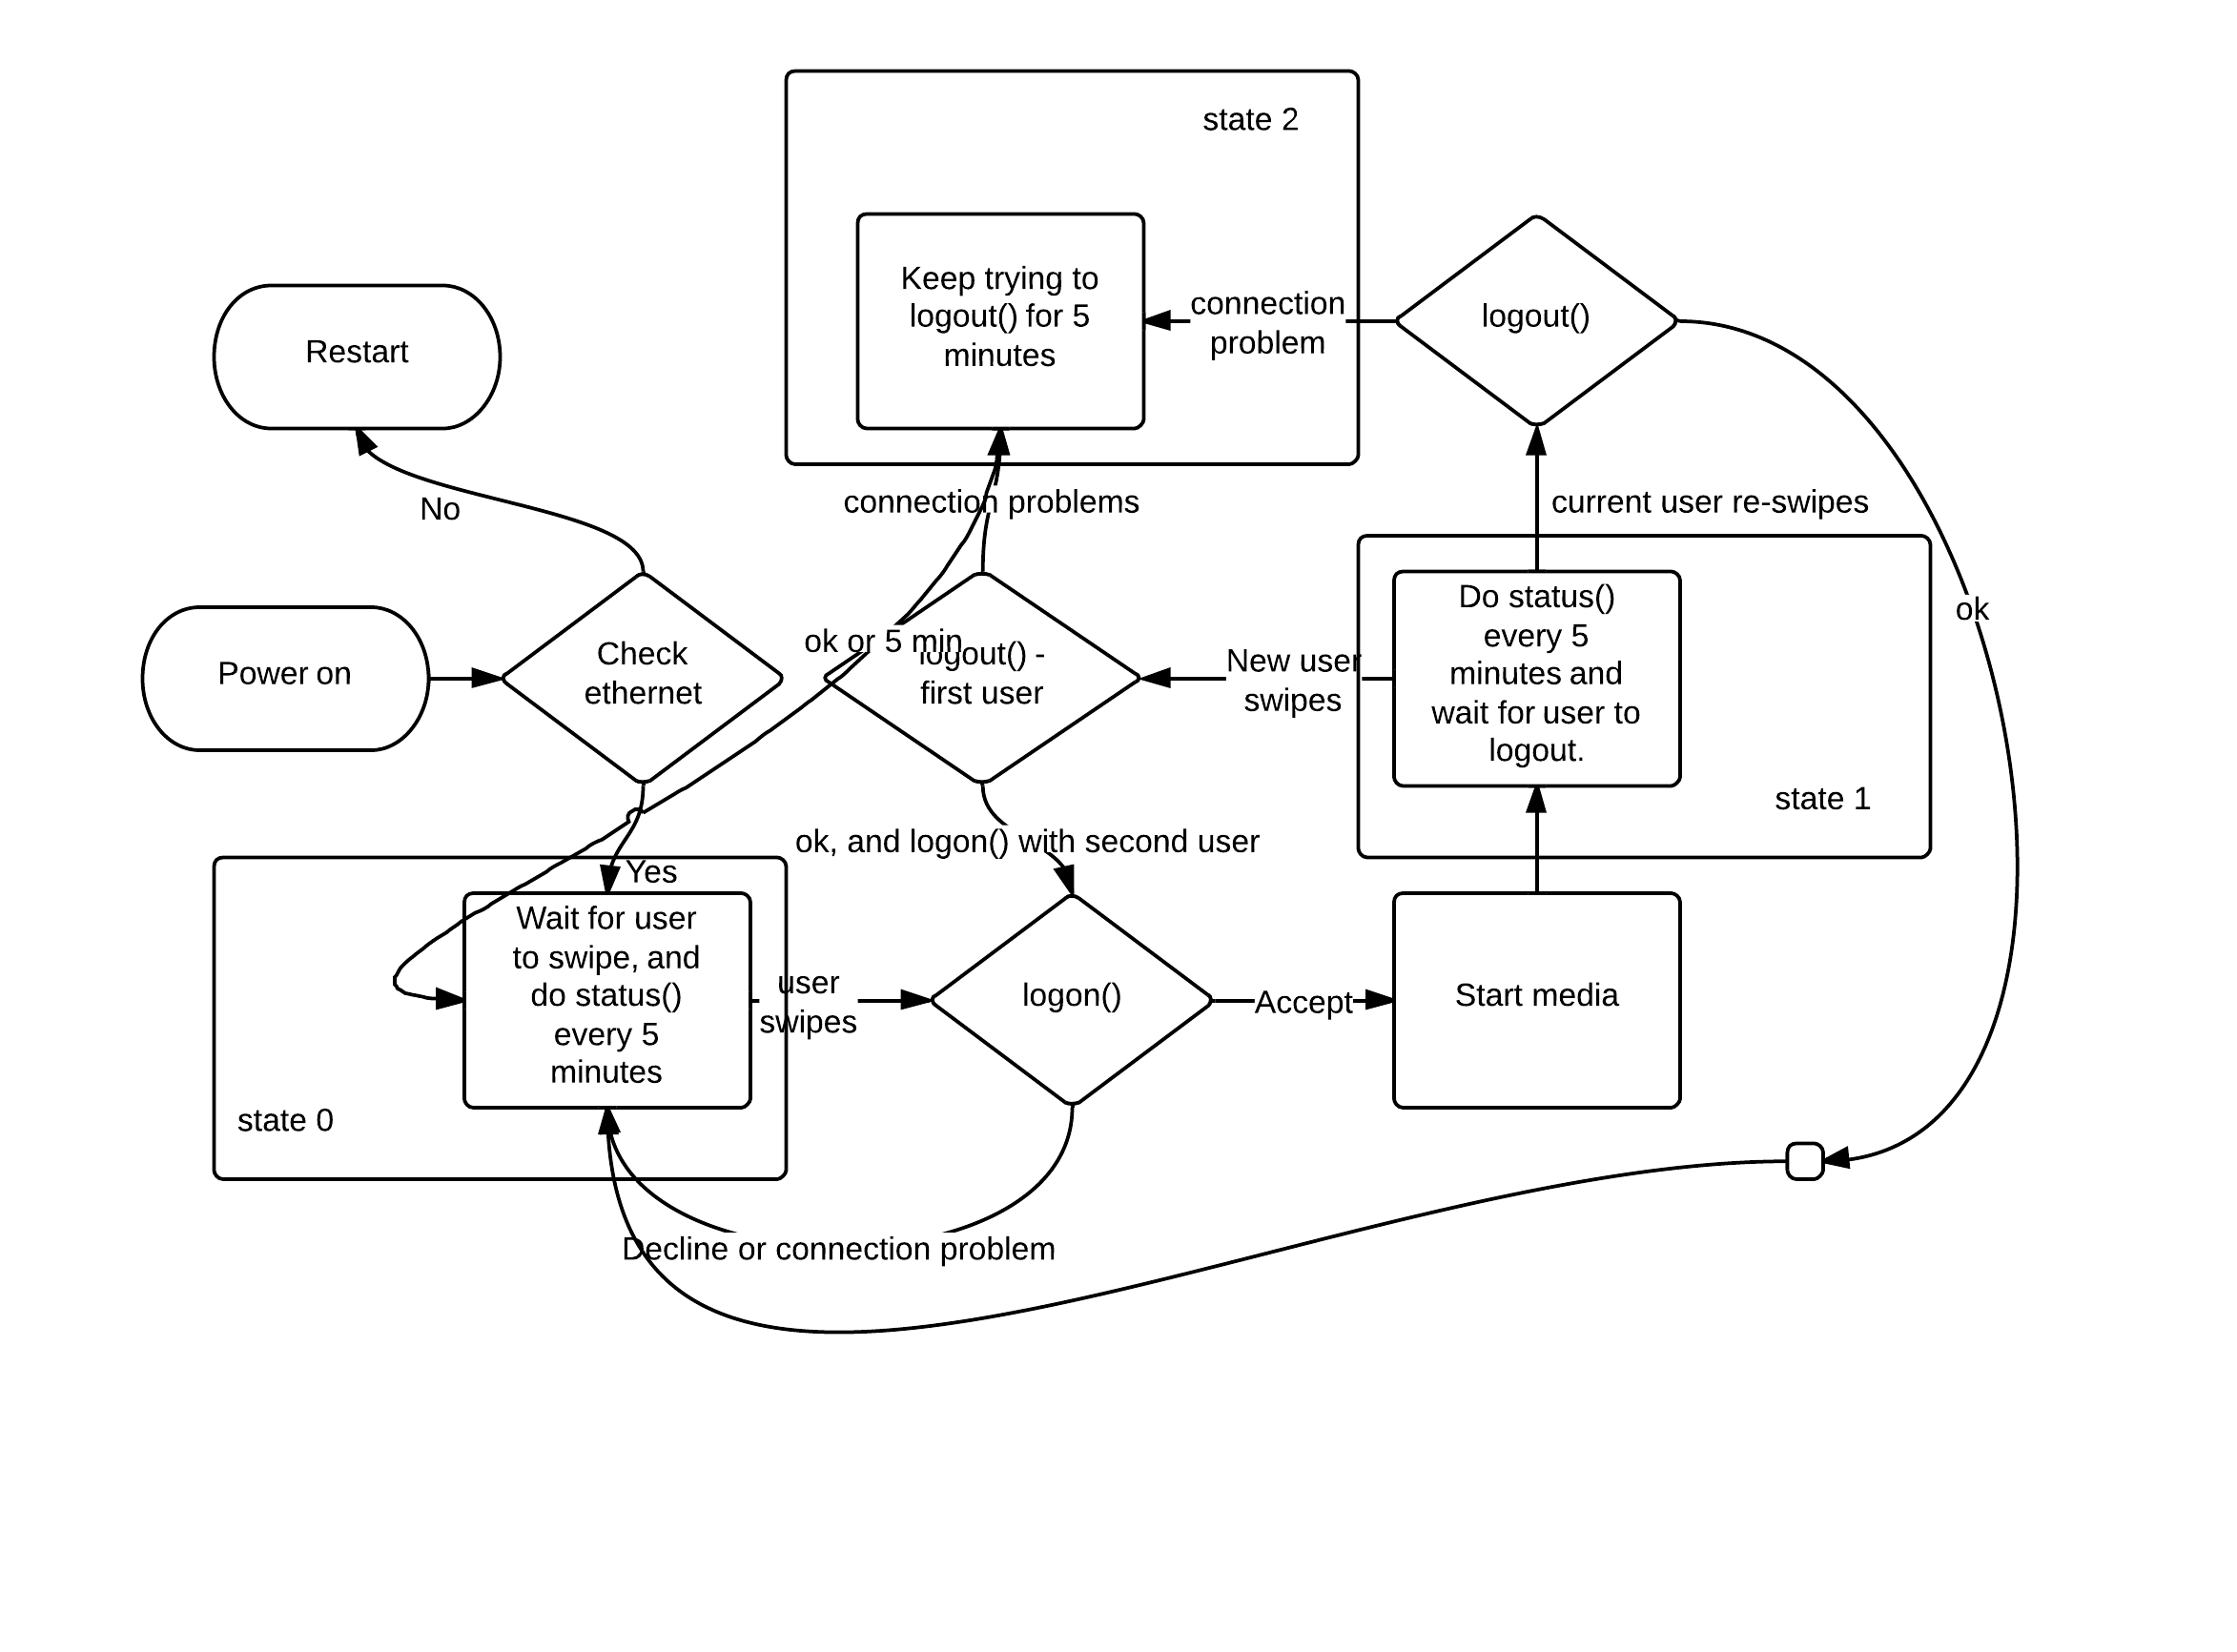
\includegraphics{images/arduinoFlowchart.png}
	\caption{Simple Flowchart of Arduino}
	\label{fig:arduinoFlowchart}
\end{figure}

As descriped in section \ref{chap:controller} is only parts of the visioned system implementet in the Arduino. 
To illustrate and describe this functionality is Figue \ref{fig:arduinoFlowchart} simpelfied flowchart and a  short describetion of the Arduino. The boxes of state in the Arduino floxchart will be described in section \ref{ProgrammingBasicsforArduino}.
The functions that was in focus to implement on the Arduino is: 

\begin{itemize}
	\item Read and accept/decline tags in communication with a server though a online connection.
	\item Monitor and handel the server connection.
	\item Regulate the power recording to the scenario.
	\item Manage the time usage and user restrictions. 
	%\item Communicate system status to user though LED light indication. 
\end{itemize}

Starting up the Arduino is setting up the ethernet connection and the pins to lights and RFID shield. If the connection can't be establehed will the Arduino needed to be restarted. This start up phase is not similar with the expected setting up phase described in \ref{subsec:senarioD} and shall therefor not be evaluatet as the end system solution.

The main time of the system is looking for tags, checking user restiction and every 5 minutes recieving updates from the database server thrugh a \verb|getStatus()| call. \\
The status call keeps the Arduino updatet on change in rules or time the user may spent at the devise.      
For most senarios of disconection from the server will resault the Arduino return to this state. 
Disconnection at log out will in a 5 minutes where the Arduino keep trying the log out procedure until accomplished else just contiue because the server at that point will have logged the user off.
Almost the same senario is when a disconnection happens at status call with a user logged on. Then the Arduino have 3 minutes to reconnect before logging off the user. 

The system is capable to switch users on the Arduino side of the MOM system. But as you may have discovered will a other user shout down the media devise the current user's use eventhough the new user don't have promission to use the media. The solution is decribed in the user senario re\ref{Logonlogoffmedia} where the API control the permission of the new user before the Arduino takes action.       
